\documentclass[twoside]{report}

%%%%% ADDED TO SUPPORT TT BOLD FACES %%%%
\DeclareFontShape{OT1}{cmtt}{bx}{n}{<5><6><7><8><9><10><10.95><12><14.4><17.28><20.74><24.88>cmttb10}{}
\renewcommand{\ttdefault}{pcr}
%%%%% END %%%%%%%%%%%%%%%%%%%%%%%%%%%%%%% 
\usepackage{atbegshi,picture}
\AtBeginShipout{\AtBeginShipoutUpperLeft{%
  \put(\dimexpr\paperwidth-1cm\relax,-1.5cm){\makebox[0pt][r]{
\includegraphics[width=3cm]{figs/inno}}}%
}}


\usepackage[english]{babel}
\usepackage{blindtext}
\usepackage{pdfpages}
\newenvironment{bottompar}{\par\vspace*{\fill}}{\clearpage}

\usepackage{cite}
\usepackage{amsmath,amsfonts}

\usepackage{amsthm}
\newtheorem{theorem}{Theorem}
\newtheorem{corollary}{Corollary}
\newtheorem{lemma}{Lemma}
\newtheorem{proposition}{Proposition}
\theoremstyle{definition}
\newtheorem{definition}{Definition}
\theoremstyle{remark}
\newtheorem*{remark}{Remark}
\theoremstyle{remark}
\newtheorem*{example}{Example}



\usepackage{float}
\usepackage{graphicx}
\usepackage{array}
\usepackage{multirow,array}
\usepackage{caption}
\usepackage{subcaption}
\usepackage{hyperref}
\usepackage{paralist}
\usepackage{listings}
\usepackage{zed-csp}
\usepackage{fancyheadings}
\usepackage{color}

\usepackage{upgreek} 
\usepackage{bm}
\usepackage{hyperref}
\usepackage{setspace}
\usepackage{booktabs}
\usepackage{multirow}
\usepackage{longtable}
\usepackage[font=singlespacing, labelfont=bf]{caption}


\usepackage{enumitem}
\newlist{inlinelist}{enumerate*}{1}
\setlist*[inlinelist,1]{%
  label=(\arabic*),
}




\pagestyle{fancyplain}

% remember section title
\renewcommand{\chaptermark}[1]%
	{\markboth{\chaptername~\thechapter~--~#1}{}}

% subsection number and title
\renewcommand{\sectionmark}[1]%
	{\markright{\thesection\ #1}}

\rhead[\fancyplain{}{\bf\leftmark}]%
      {\fancyplain{}{\bf\thepage}}
\lhead[\fancyplain{}{\bf\thepage}]%
      {\fancyplain{}{\bf\rightmark}}
\cfoot{} %bfseries


\newcommand{\dedication}[1]
   {\thispagestyle{empty}
     
   \begin{flushleft}\raggedleft #1\end{flushleft}
}

\begin{document}\sloppy

%NOTE:
% change the title of your thesis
% titles/BS.pdf for Bachelor (default)
% titles/DS.pdf for Master in Data Science
% titles/Rob.pdf for Master in Robotics
% titles/SE.pdf for Master in Software Engineering
% titles/SNE.pdf for Master in Security and Network Engineering 

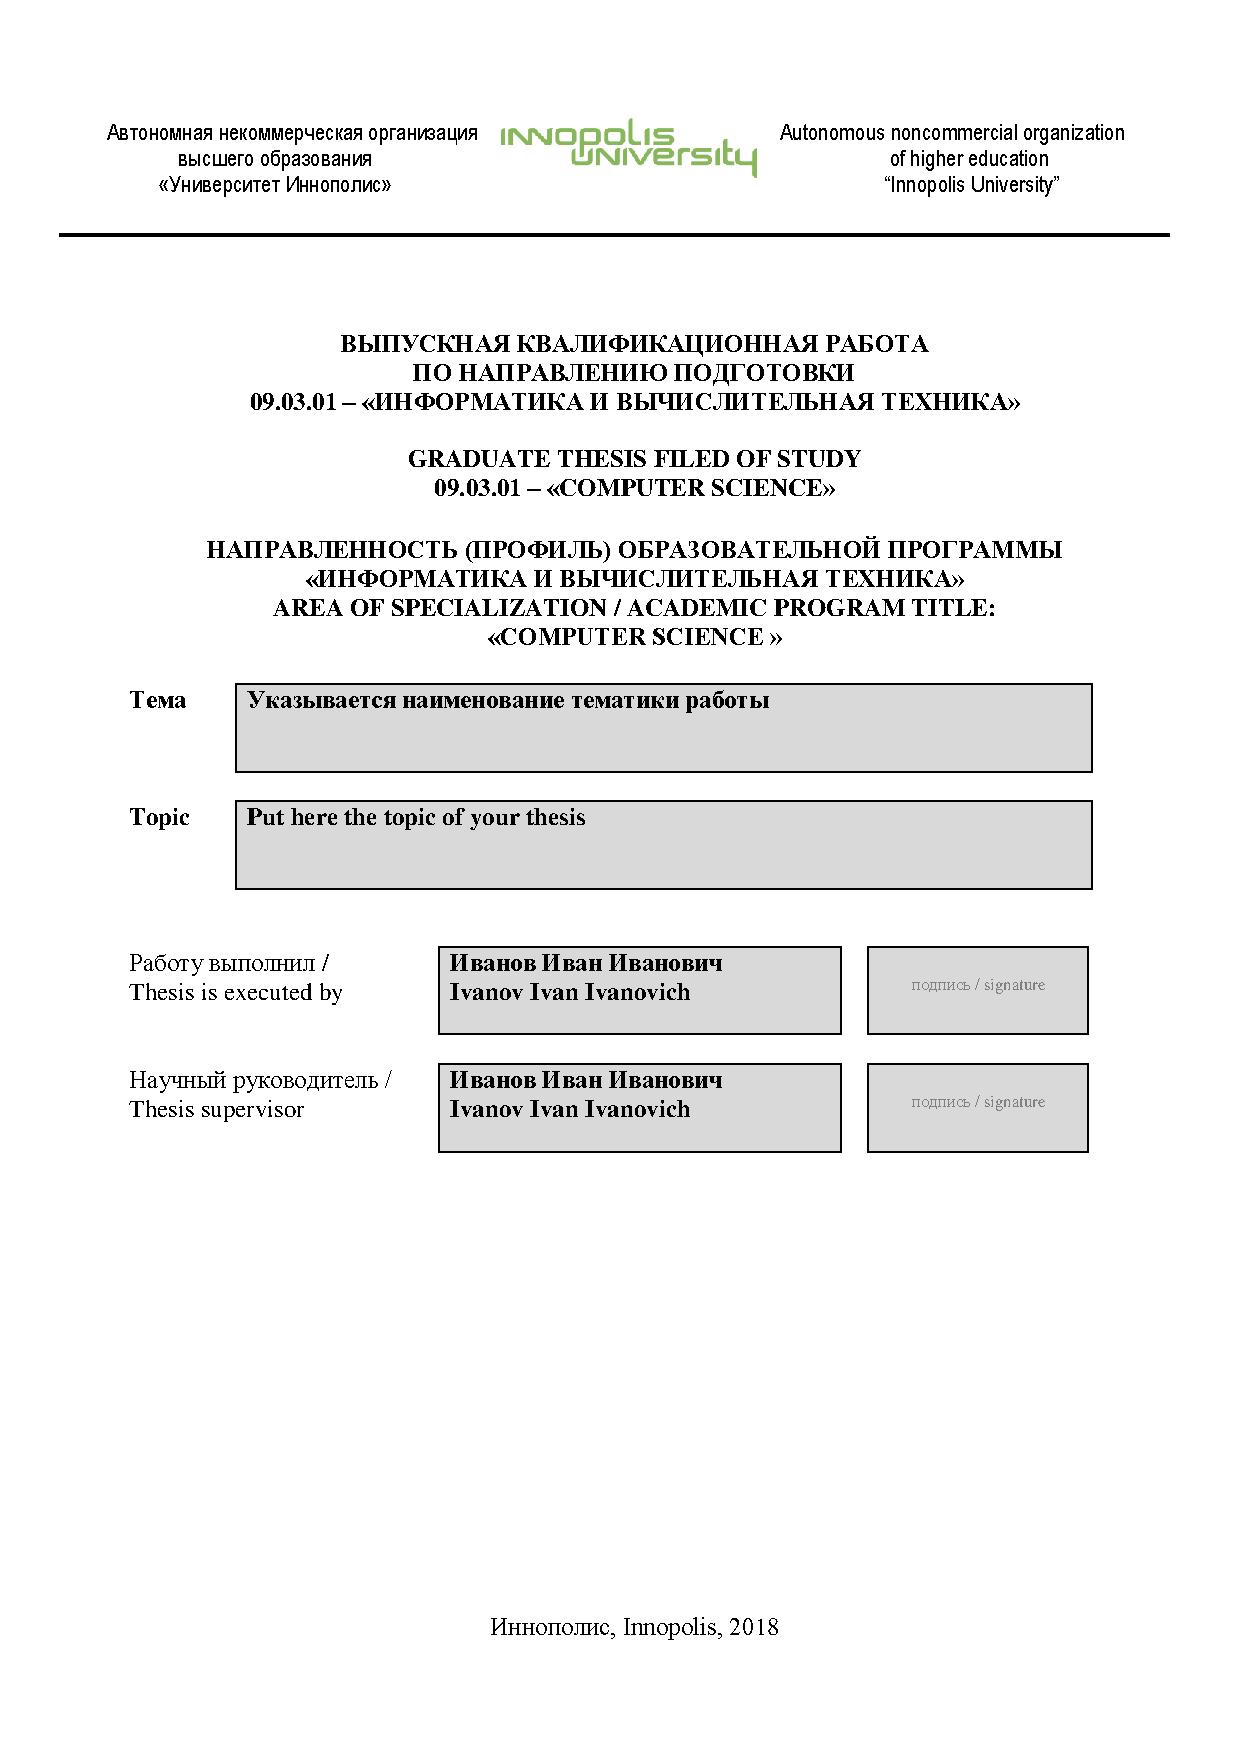
\includepdf[pages=-]{titles/BS.pdf}
\newpage
\dedication{(optional) dedication.}
\newpage
\setcounter{page}{5}

\newpage
\thispagestyle{empty}
\mbox{}

\newpage

\tableofcontents
\listoftables
\listoffigures

\newpage
\begin{abstract}
abstract \ldots
\end{abstract}

%!TEX root = root.tex

\chapter{Introduction}
\label{chap:intro}
\chaptermark{Optional running chapter heading}

\section{Spacing \& Type}
\label{sec:section}

This is a section. This is a citation without brackets \citen{A}. and this is one with brackets \cite{A}. These are multiple citations: [\citen{A, B, C}]. Here's a reference to a subsection: \ref{sec:subsection}. The body of the text and abstract must be double-spaced except for footnotes or long quotations. Fonts such as Times Roman, Bookman, New Century Schoolbook, Garamond, Palatine, and Courier are acceptable and commonly found on most computers. The same type must be used throughout the body of the text. The font size must be 10 point or larger and footnotes\footnote{This is a footnote.} must be two sizes smaller than the text\footnote{This is another footnote.} but no smaller than eight points. Chapter, section, or other headings should be of a consistent font and size throughout the ETD, as should labels for illustrations, charts, and figures.  

\subsection{Creating a Subsection}
\label{sec:subsection}

\subsubsection{Creating a Subsubsection}

\paragraph{This is a heading level below subsubsection}

And this is a quote: 
%
\begin{quote}
\blindtext
\end{quote}

This is a table:
% currsize is not set in the long table environment, so we need to set it before we set it up.
\makeatletter
\let\@currsize\normalsize
\makeatother

% tabular environments are set to be single-spaced in the  thesis class,  but long tables do not use tabular
% to get around this, set the spacing to single spacing at the start of the long table environment, and set it back to double-spacing at the end of it

\begin{longtable}{cc}
\caption[This is the title I want to appear in the List of Tables]{This is a caption.} \label{tab:pfams} \\
\hline
A & B \\
\hline
\endfirsthead
\multicolumn{2}{@{}l}{\textbf{Table \thetable} \ldots continued} \\
\hline
A & B \\
\hline
\endhead
a1 & b1 \\
a2 & b2 \\
a3 & b3 \\
a4 & b4 \\
\hline
\end{longtable}


The package ``upgreek'' allows us to use non-italicized lower-case greek letters. See for yourself: $\upbeta$, $\bm\upbeta$, $\beta$, $\bm\beta$. Next is a numbered equation:
\begin{align}
\label{eq:name}
\|\bm{X}\|_{2,1}={\underbrace{\sum_{j=1}^nf_j(\bm{X})}_{\text{convex}}}=\sum_{j=1}^n\|\bm{X}_{.,j}\|_2
\end{align}
The reference to equation (\ref{eq:name}) is clickable. 

\section[Theorems, Corollaries, Lemmas, Proofs, Remarks, Definitions\\ and Examples]{Theorems, Corollaries, Lemmas,\\ Proofs, Remarks, Definitions,\\ and Examples}

\begin{theorem}
\label{thm:onlytheorem}
\blindtext
\end{theorem}

\begin{proof}
I'm a (very short) proof.
\end{proof}

\begin{lemma}
I'm a lemma.
\end{lemma}

\begin{corollary}
I include a reference to Thm. \ref{thm:onlytheorem}.
\end{corollary}

\begin{proposition}
I'm a proposition.
\end{proposition}

\begin{remark}
I'm a remark. 
\end{remark}

\begin{definition}
I'm a definition. I'm a definition. I'm a definition. I'm a definition. I'm a definition. I'm a definition. I'm a definition. I'm a definition. I'm a definition. I'm a definition. I'm a definition. 
\end{definition}

\begin{example}
I'm an example.
\end{example}


\section[Optional table of contents heading]{Section with\\ linebreaks in\\the
name}


\Blindtext[2]





\chapter{Literature Review}
\label{chap:lr}
\chaptermark{Second Chapter Heading}

%\Blindtext[2]

\section{RNN Encoder-decoder}

\cite{B}

\begin{align}
\label{prob-trans}
\ p(y) = \prod_{t=1}^{T} p(y_t | \{y_1, \dots, y_{t-1}\}, c),
\end{align}
where $y = (y_1, \dots, y_{T_{y}})$. The reference to equation (\ref{prob-trans}) is clickable. 

\section{Attention}
Introduction of recurrent neural network encoder-decoder architecture has revolutionised machine translation. However, they have suffered from one critical flaw: deterioration of performance with increasing of input sentence length\cite{C}. Authors have evaluated Encoder–Decoder against baseline phrase-based statistical model Moses \cite{D} using BLEU score \cite{E}. The results have demonstrated clear degradation of performance on longer sentences. The authors hypothesize that this issue is caused by scarcity of fixed-length vector's capacity to encode a long sentence with complicated structure and meaning.

This bottleneck was addressed in \cite{A}. The authors have introduced an approach which encodes the input sequence into a sequence of vectors, annotations. They are used in decider choose parts of the sentence it should pay attention to. This approach relieves the encoder from burden of capturing information about whole source sentence.

The attention mechanism provides new formula for conditional probability of getting next word of translation $y_i$ given previously predicted words:
\begin{align}
\label{att-prob}
\ p(y_i| y_1, \dots, y_{i-1}, x) = g(y_{i-1}, s_i, c_i),
\end{align}
where $s_i$ is an RNN hidden state for time i:
\begin{align}
\ s_i = f(s_{i-1}, y_{i-1}, c_i).
\end{align}

\begin{figure}[H]
\centering
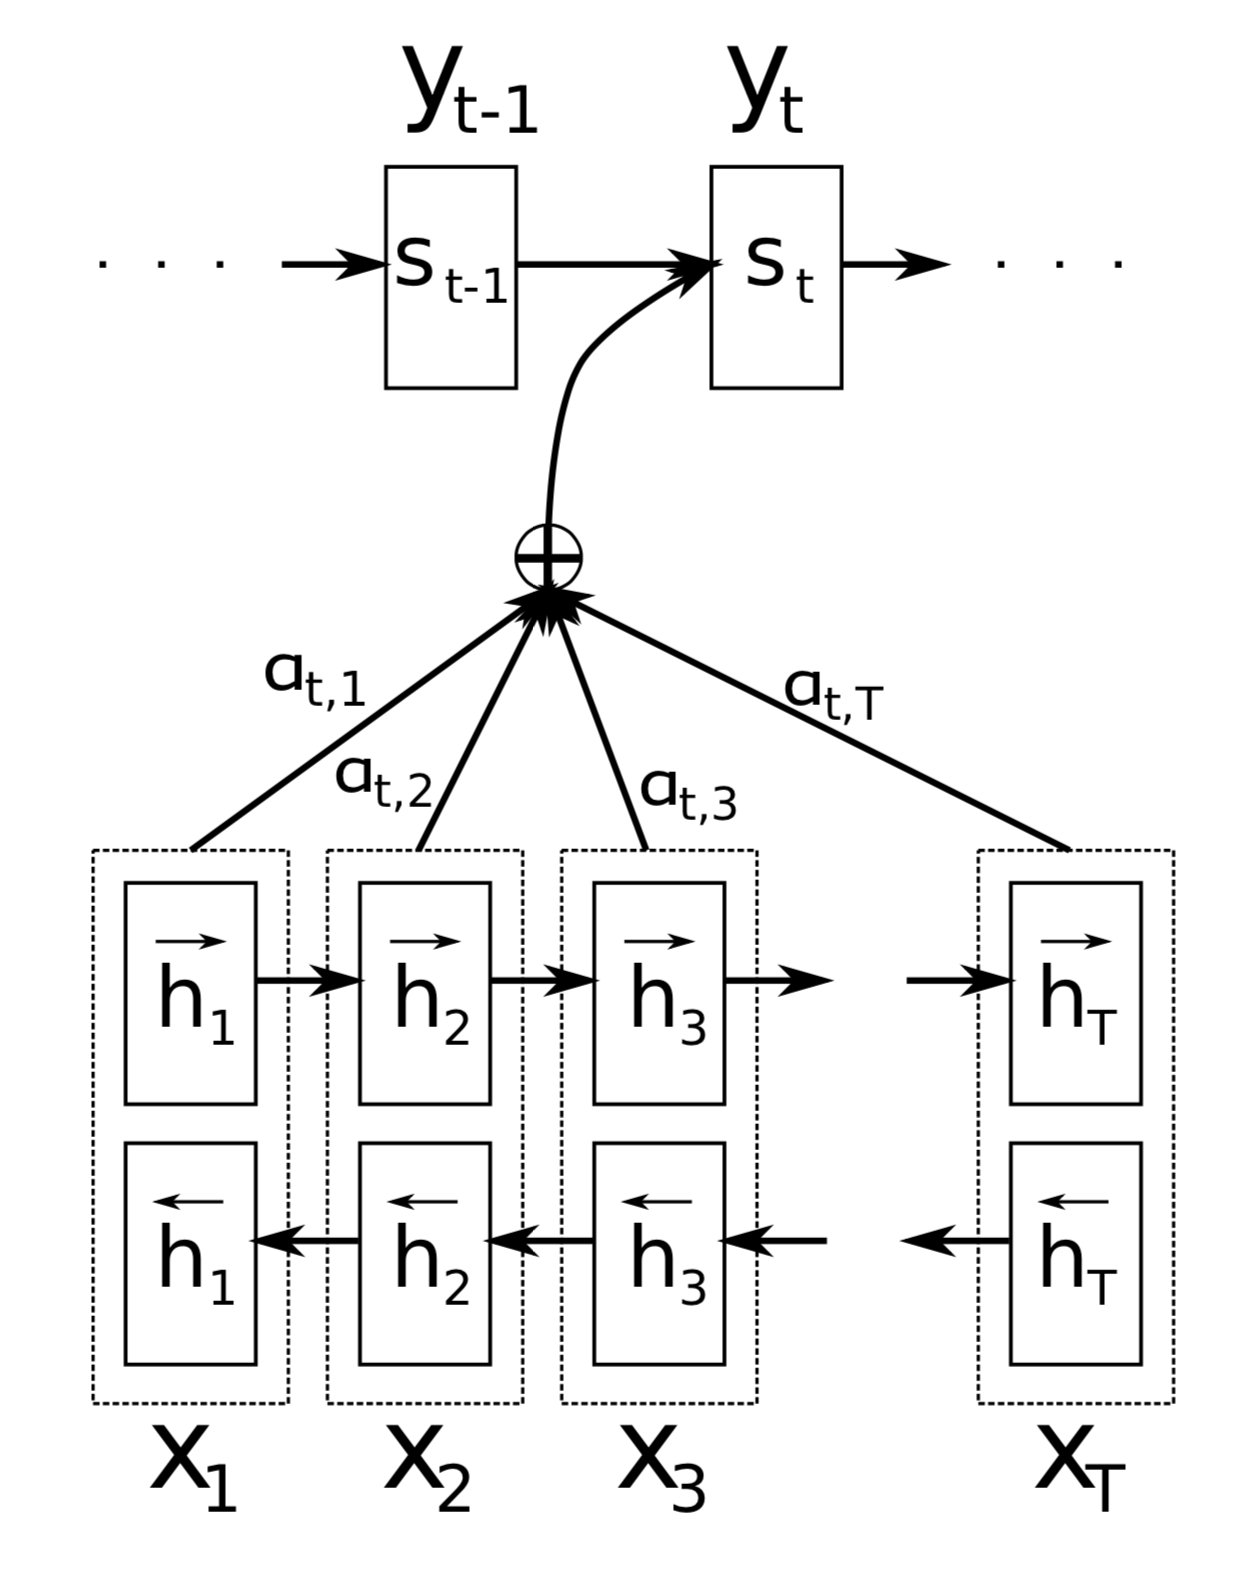
\includegraphics[width=0.3\textwidth]{figs/attention.png}
\caption[Attention model illustration]{Attention model illustration.}
\label{att-ill}
\end{figure}

The Figure \ref{att-ill} illustrates the proposed model generating the $t$th target word $y_t$ given a source sentence $(x_1,x_2,...,x_T )$.

The encoder is used to calculate sequence annotations and consists of two RNNs: backward and forward. This is done to capture both preceding and following words. Reading the sequence from both directions results in two sets of RNNs' hidden states: forward - $(\overrightarrow{h_1}, \dots, \overrightarrow{h_{T_x}})$; and backward - $(\overleftarrow{h_1}, \dots, \overleftarrow{h_{T_x}})$. Each pair of corresponding vectors is concatenated to form a final set of sequence annotations: $h_j = [\overrightarrow{h_j}; \overleftarrow{h_j}]^T$.

Each context $c_i$ is computed as a weighted sum of sequence of annotations $(h_1, \dots, h_{T_{x}})$:

\begin{align}
\label{cont-vec}
\ c_i = \sum_{j=1}^{T_x} \alpha_{ij}h_j.
\end{align}

The weight $\alpha_{ij}$ of each annotation $h_j$ is computed by

\begin{align}
\label{ann-weight}
\ \alpha_{ij} = \frac{exp(e_{ij})}{\sum_{k=1}^{T_x}exp(e_{ik})},
\end{align}
where
\begin{align}
\ c_{ij} = a(s_{i-1}, h_j).
\end{align}
is an alignment model that evaluates how well the inputs around position $j$ and the $i$th output match. It is parametrized as a feedforward neural network. Each weight can be seen as a probability that the target word $y_i$ is aligned to a source word $x_j$, and it reflects the importance of annotation with respect to a previous hidden state in generating next output word $y_i$ and deciding the next state. This implements a mechanism of attention in decoder, which lets it decide the most important part of source sentence for each step of translation. 

%\Blindtext[1]

\chapter{Methodology}
\label{chap:met}


\ldots

Referencing other chapters \ref{chap:lr}, \ref{chap:met}, \ref{chap:impl}, \ref{chap:eval} and \ref{chap:conclusion}

\ldots
\chapter{Implementation}
\label{chap:impl}


\ldots

\chapter{Evaluation and Discussion}
\label{chap:eval}


\ldots

\chapter{Conclusion}
\label{chap:conclusion}


\ldots



%% REFERENCES
\bibliographystyle{apalike}
\bibliography{thesis}
\appendix
\chapter{Extra Stuff}
\blindtext

\chapter{Even More Extra Stuff}
\blindtext
\end{document}

